\section{The landscape of space situational awareness}

The near-Earth space environment has experienced an unprecedented densification over the last decade. With the advent of massive satellite constellations and the compounding accumulation of orbital debris, space situational awareness has transitioned from a monitoring exercise into a critical, high-frequency computational challenge. Simultaneously, the modern geopolitical and scientific focus has rapidly expanded outwards to the cislunar domain, the vast, complex region of space encompassing the Earth, the Moon, and the Lagrange points that balance their gravitational pulls. 

Driven by international initiatives like the Artemis programme and the Lunar Gateway, the cislunar environment is slated to become the next major frontier for human presence and autonomous satellite operations. Both of these regimes demand a fundamental paradigm shift in how we track resident space objects. In near-Earth orbit, operators must rigorously track the evolution of probability density functions over time to accurately assess collision probabilities. In the cislunar environment, modelling continuous multi-body gravitational interactions results in highly non-linear dynamics where trajectories are incredibly sensitive to initial conditions.

Consequently, the deterministic tracking of satellites, representing them as single, certain points in space, is not sufficient. To maintain safe operations, prevent collisions, and ensure mission viability across all orbital regimes, astrodynamicists are transitioning from tracking singular points to propagating entire clouds of uncertainty.

\section{The breakdown of Gaussian assumptions} \label{sec:gaussian_breakdown}

The state of an object in orbit is most commonly parameterised using a set of coordinates known as the \emph{equinoctial} elements, which are six-dimensional. This coordinate system resolves the mathematical singularities inherent in classical \emph{Keplerian} elements. However, propagating probability distributions through the highly non-linear dynamics of orbital mechanics introduces significant analytical difficulties. While the initial uncertainty of a satellite's state immediately following an observation might be well-approximated by a multivariate Gaussian distribution, the true physical distribution rapidly distorts as the states are propagated forward in time. 

The primary driver of this distortion is the physical ground truth shear of the orbital environment. Differential gravitational effects, atmospheric drag, and solar radiation pressure collectively induce non-linear shearing on the state space. As the uncertainty cloud is pushed through these dynamics, it stretches, folds, and develops heavy tails, frequently exhibiting distinct ``boomerang" or highly coupled geometries~\cite{Horwood2014}.

\begin{figure}
    \centering
    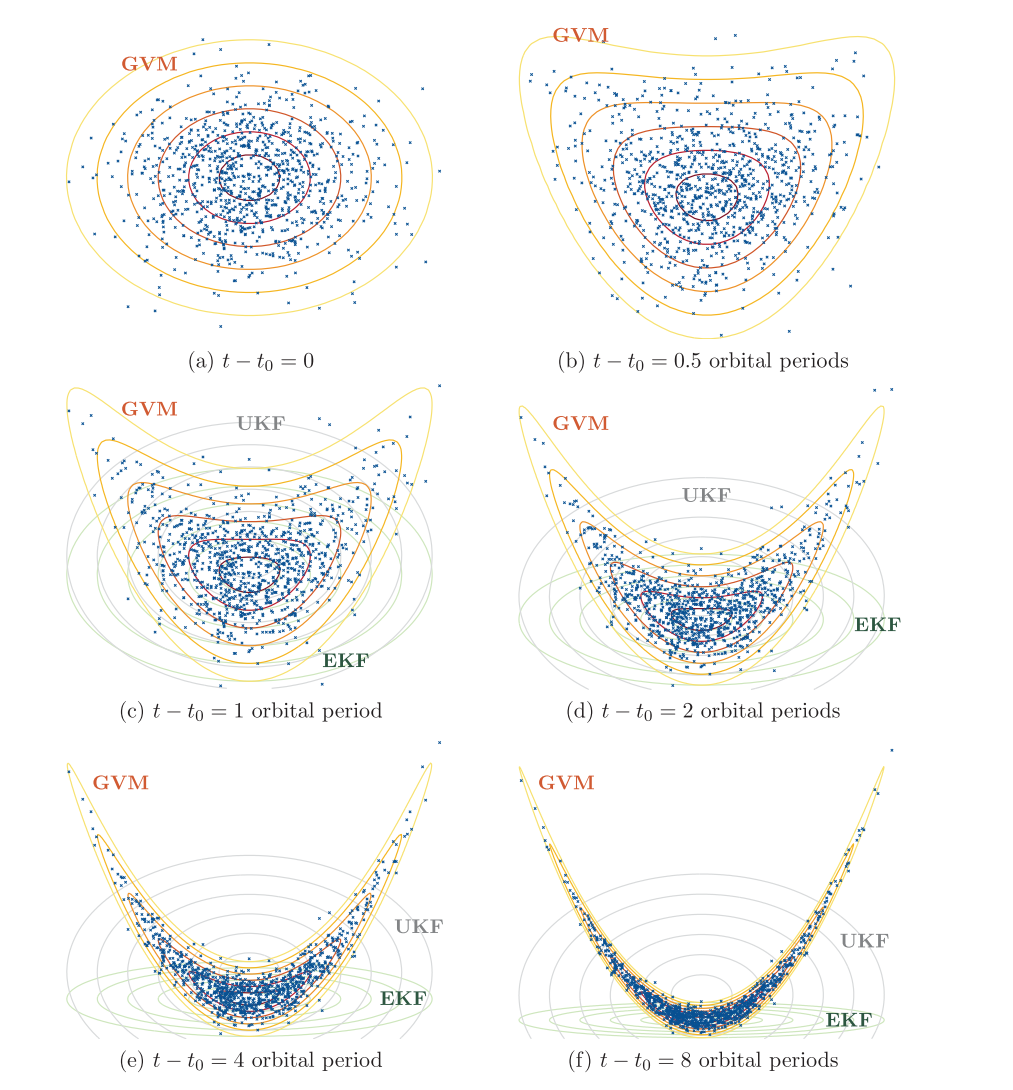
\includegraphics[width=\linewidth]{figures/Horwood_distributions.png}
    \caption{Evolution of equinoctial elements across propagation epochs~\cite{Horwood2014}.}
    \label{fig:horwood_distributions}
\end{figure}

Classical filtering techniques, such as the Extended Kalman Filter (EKF) and the Unscented Kalman Filter (UKF), are fundamentally ill-equipped to handle these dynamics over extended time horizons. These methods implicitly assume that the underlying probability distribution remains at least approximately Gaussian. Constraining the propagated uncertainty within a linearised Gaussian covariance ellipsoid fundamentally mischaracterises the underlying non-linear dynamical flow. By forcing this rigid geometry over a highly sheared physical distribution, classical filters frequently position their maximum likelihood estimate entirely outside the support of the true state~\ref{fig:horwood_distributions}. Consequently, the filter erroneously assigns peak probability density to regions of the state space where the actual physical measure is strictly zero.

This effect is visualised in Figure~\ref{fig:horwood_distributions}, where a particle cloud approximating a set of low-Earth equinoctial orbital elements is forward-propagated over several orbital periods. Three probability distributions are fitted to these data, namely two Gaussians emanating from the EKF and UKF, respectively, and a Gauss Von Mises (GVM) distribution, which more accurately models the nonlinear shearing of the orbital elements (more in Chapter~\ref{ch:experiments_and_applications}). A two-dimensional slice along the semi-major axis--mean longitude plane is then plotted alongside each of the three probability contours. From Figure~\ref{fig:horwood_distributions}, it is clear that the GVM distribution strongly outperforms the EKF and UKF over long-term propagation. This divergence between assumed mathematical models and physical reality necessitates a different approach to uncertainty modelling, one that can embrace and accurately represent arbitrary non-Gaussian distributions.

\section{Optimal transport and triangular maps}

To capture the complex, sheared distributions dictated by orbital mechanics, we turn to the mathematical theory of optimal transport. Originating from the problem of finding the most efficient way to move piles of earth to fill construction trenches~\cite{monge1781memoire}, this discipline provides a rigorous framework for defining a continuous mathematical map that pushes a simple, easy-to-sample reference distribution onto a more complex target distribution (such as that discussed in Section~\ref{sec:gaussian_breakdown}).

Instead of propagating the physical probability measure directly through the non-linear dynamical flow, optimal transport frames the uncertainty quantification problem as learning a continuous pushforward map between two distinct probability spaces. This deterministic transformation acts as a structural bridge, coupling a tractable, well-characterised reference measure, such as an isotropic standard Gaussian, directly to the highly complex, sheared target distribution dictated by the physical ground truth. By accurately reconstructing this map, we can bypass the local linearisation flaws of classical filters. We can draw vast ensembles of independent, identically distributed samples from the simple reference space, push them forward through our learned map, and thus recover the true, heavy-tailed non-Gaussian geometry of the evolved physical uncertainty cloud.

% However, discovering a general optimal transport map in a high-dimensional setting is inherently challenging; without structural restrictions, the computational cost of searching for an arbitrary mapping grows restrictively large as the state space expands. To render the problem computationally tractable, one can impose a structural constraint on the transformation by seeking a \emph{triangular map}. Instead of attempting to map the entire multi-dimensional space simultaneously, this map decomposes the problem by imposing a lower-triangular structure, dictating that each successive dimension of the state vector is constructed using only the information from the dimensions that preceded it. By mirroring the natural, step-by-step conditional dependencies of the physical system, the triangular formulation serves as an ideal framework for tracking the cascading, coupled uncertainties present in orbital mechanics.

\section{Computational challenges}

While triangular maps provide an elegant theoretical framework for probability transport, translating this continuous abstraction into a functional computational tool introduces significant engineering challenges. In learning multi-dimensional maps, first-order optimisation methods such as projected gradient descent (PGD) offer significant computational advantages over more sophisticated frameworks such as quasi-Newton or interior-point methods used in the literature~\cite{Baptista2022}.

In the PGD framework we propose in this thesis, to preserve the physical validity of the transported probability distribution, the learned map must remain strictly monotonic. This requirement manifests as a large number of linear inequality constraints, defining a strict permissible region for the map's parameters. Geometrically, this space of valid parameters forms a sparse, multi-dimensional polyhedron. Whenever the PGD algorithm pushes the parameters outside the valid region, they must be mathematically mapped back to the closest point on the boundary of the polyhedron. This fundamental operation is known as a Euclidean projection.

\section{Dykstra's algorithm and stalling}

Since we require a Euclidean projection at every single epoch of a high-frequency learning loop, the choice of projection algorithm dictates the overall viability of the tracking framework. Standard interior-point optimisation software is often computationally prohibitive for such large-scale, high-dimensional tasks. Dykstra's projection algorithm offers a computationally inexpensive, scalable solution to compute these Euclidean projections. Utilised across various engineering disciplines---such as restricted least squares in machine learning or model predictive control---Dykstra's algorithm breaks down the (often intractable) joint projection into a sequence of simple iterative steps, offering phenomenally low per-iteration computational overhead.

However, Dykstra's algorithm harbours a fatal mathematical flaw known as the stalling phenomenon. In specific geometric configurations, particularly near the sharp, complex intersections of multiple constraint planes, the iterates can be subject to arbitrarily long cycles. During these unpredictable stalling periods, the algorithm stops moving towards the true optimal projection. In safety-critical or real-time applications, where a fixed iteration budget is utilised to satisfy computational constraints (such as our optimal transport framework), the stalling phenomenon can completely inhibit the feasible deployment of Dykstra's algorithm. Furthermore, the standard ``vanilla'' implementation of this algorithm lacks any optimisation enhancement, a gap that must be closed to allow Dykstra's integration in space-ready software.

\section{Summary of contributions}

This thesis bridges the gap between fundamental algorithmic optimisation and high-dimensional physical modelling. As a cross-disciplinary effort between the Operations Research and Financial Engineering (ORFE) and the Mechanical and Aerospace Engineering (MAE) departments, the core contributions of this work are explicitly dual in nature, forming two distinct yet interconnected main sections.

First, we resolve the known stalling phenomenon in Dykstra's algorithm. By rigorously analysing the geometry of polyhedral constraints, we derive an exact, closed-form mathematical solution for the duration of the stalling period. Building upon this derivation, we introduce a fast-forward modification to the algorithm. When a stall is detected, a single, computationally inexpensive update instantly advances the internal memory variables to the end of the stall. Alongside several other optimisation enhancements, these modifications eliminate the unpredictable convergence behaviour of the algorithm while preserving its strong asymptotic convergence guarantees, transforming it into a highly robust engine for real-time and safety-critical engineering applications.

Second, we architect a scalable software framework for optimal transport in orbital mechanics. Leveraging the fast-forward modified Dykstra solver, we construct a robust PGD framework to learn triangular maps. By successfully reconstructing non-linear physical ground truth shears, we establish this combined engine as a viable, highly performant alternative to traditional filtering. Ultimately, we demonstrate that optimal transport, when coupled with rigorous mathematical optimisation, can fundamentally advance the state-of-the-art in space domain awareness. This applied framework paves the way for dynamically tracking complex, non-Gaussian uncertainty distributions across diverse orbital regimes, providing a critical computational tool for ensuring safe, reliable, and autonomous operations in the modern space environment.

\section{Thesis outline}

The remainder of this thesis is structured as follows. 

Chapter~\ref{ch:dykstra} focuses on the theoretical advancements to Dykstra's projection algorithm. It introduces the geometry of Euclidean projections and polyhedral sets, formally defines the stalling phenomenon, and presents the mathematical proof for the closed-form duration of the stall. The chapter concludes by defining the fast-forward modified algorithm and demonstrating its superiority on pathological constraint geometries.

Chapter~\ref{ch:optimal_transport} pivots to the aerospace application, formally defining the theory of optimal transport and the structure of triangular maps. It details the parameterisation of these maps and formulates the monotonicity requirements into a constrained optimisation problem.

Chapter~\ref{ch:optimisation} details the architecture of the custom Python software framework. It outlines the integration of the outer learning loop, featuring stochastic gradient descent and several other dynamic learning schedules.

Chapter~\ref{ch:experiments_and_applications} presents the empirical results of applying the framework to orbital mechanics and geophysical applications. It features the successful reconstruction of physical ground truth shears and provides performance scaling metrics demonstrating the computational efficiency of the combined architecture. 

Finally, Chapter~\ref{ch:conclusion} summarises the primary findings, details the broader implications for both the optimisation and astrodynamics communities, and proposes avenues for future theoretical and applied work.